\ifx\wholebook\relax \else
% ------------------------ 

\documentclass{article}
%------------------- Other types of document example ------------------------
%
%\documentclass[twocolumn]{IEEEtran-new}
%\documentclass[12pt,twoside,draft]{IEEEtran}
%\documentstyle[9pt,twocolumn,technote,twoside]{IEEEtran}
%
%-----------------------------------------------------------------------------
%%
% loading packages
%
\newif\ifpdf
\ifx\pdfoutput\undefined % We're not running pdftex
  \pdffalse
\else
  \pdftrue
\fi
%
%
\ifpdf
  \RequirePackage[pdftex,%
            CJKbookmarks,%
       bookmarksnumbered,%
              colorlinks,%
          linkcolor=blue,%
              hyperindex,%
        plainpages=false,%
       pdfstartview=FitH]{hyperref}
\else
  \RequirePackage[dvipdfm,%
             CJKbookmarks,%
        bookmarksnumbered,%
               colorlinks,%
           linkcolor=blue,%
               hyperindex,%
         plainpages=false,%
        pdfstartview=FitH]{hyperref}
  \AtBeginDvi{\special{pdf:tounicode GBK-EUC-UCS2}} % GBK -> Unicode
\fi
\usepackage{hyperref}

% other packages
%-----------------------------------------------------------------------------
\usepackage{graphicx, color}
\usepackage{CJK}
%
% for programming 
%
\usepackage{verbatim}
\usepackage{listings}


\lstdefinelanguage{Smalltalk}{
  morekeywords={self,super,true,false,nil,thisContext}, % This is overkill
  morestring=[d]',
  morecomment=[s]{"}{"},
  alsoletter={\#:},
  escapechar={!},
  literate=
    {BANG}{!}1
    {UNDERSCORE}{\_}1
    {\\st}{Smalltalk}9 % convenience -- in case \st occurs in code
    % {'}{{\textquotesingle}}1 % replaced by upquote=true in \lstset
    {_}{{$\leftarrow$}}1
    {>>>}{{\sep}}1
    {^}{{$\uparrow$}}1
    {~}{{$\sim$}}1
    {-}{{\sf -\hspace{-0.13em}-}}1  % the goal is to make - the same width as +
    %{+}{\raisebox{0.08ex}{+}}1		% and to raise + off the baseline to match -
    {-->}{{\quad$\longrightarrow$\quad}}3
	, % Don't forget the comma at the end!
  tabsize=2
}[keywords,comments,strings]

\lstloadlanguages{C++, Lisp, Haskell, Python, Smalltalk}

% ======================================================================

\def\BibTeX{{\rm B\kern-.05em{\sc i\kern-.025em b}\kern-.08em
    T\kern-.1667em\lower.7ex\hbox{E}\kern-.125emX}}

\newtheorem{theorem}{Theorem}

%
% mathematics
%
\newcommand{\be}{\begin{equation}}
\newcommand{\ee}{\end{equation}}
\newcommand{\bmat}[1]{\left( \begin{array}{#1} }
\newcommand{\emat}{\end{array} \right) }
\newcommand{\VEC}[1]{\mbox{\boldmath $#1$}}

% numbered equation array
\newcommand{\bea}{\begin{eqnarray}}
\newcommand{\eea}{\end{eqnarray}}

% equation array not numbered
\newcommand{\bean}{\begin{eqnarray*}}
\newcommand{\eean}{\end{eqnarray*}}

\RequirePackage{CJK,CJKnumb,CJKulem,CJKpunct}
% we use CJK as default environment
\AtBeginDocument{\begin{CJK*}{GBK}{song}\CJKtilde\CJKindent\CJKcaption{GB}}
\AtEndDocument{\clearpage\end{CJK*}}

%
% loading packages
%

\RequirePackage{ifpdf}

%
%
\ifpdf
  \RequirePackage[pdftex,%
       bookmarksnumbered,%
              colorlinks,%
          linkcolor=blue,%
              hyperindex,%
        plainpages=false,%
       pdfstartview=FitH]{hyperref}
\else
  \RequirePackage[dvipdfm,%
        bookmarksnumbered,%
               colorlinks,%
           linkcolor=blue,%
               hyperindex,%
         plainpages=false,%
        pdfstartview=FitH]{hyperref}
\fi
\usepackage{hyperref}

% other packages
%--------------------------------------------------------------------------
\usepackage{graphicx, color}
\usepackage{subfig}

\usepackage{amsmath, amsthm, amssymb} % for math
\usepackage{exercise} % for exercise

%
% for programming 
%
\usepackage{verbatim}
\usepackage{listings}
%\usepackage{algorithmic} %old version; we can use algorithmicx instead
\usepackage{algorithm} 
\usepackage[noend]{algpseudocode} %for pseudo code, include algorithmicsx automatically
\usepackage{makeidx} % for index support


\lstdefinelanguage{Smalltalk}{
  morekeywords={self,super,true,false,nil,thisContext}, % This is overkill
  morestring=[d]',
  morecomment=[s]{"}{"},
  alsoletter={\#:},
  escapechar={!},
  literate=
    {BANG}{!}1
    {UNDERSCORE}{\_}1
    {\\st}{Smalltalk}9 % convenience -- in case \st occurs in code
    % {'}{{\textquotesingle}}1 % replaced by upquote=true in \lstset
    {_}{{$\leftarrow$}}1
    {>>>}{{\sep}}1
    {^}{{$\uparrow$}}1
    {~}{{$\sim$}}1
    {-}{{\sf -\hspace{-0.13em}-}}1  % the goal is to make - the same width as +
    %{+}{\raisebox{0.08ex}{+}}1		% and to raise + off the baseline to match -
    {-->}{{\quad$\longrightarrow$\quad}}3
	, % Don't forget the comma at the end!
  tabsize=2
}[keywords,comments,strings]

\lstloadlanguages{C++, Lisp, Haskell, Python, Smalltalk}

% ======================================================================

\def\BibTeX{{\rm B\kern-.05em{\sc i\kern-.025em b}\kern-.08em
    T\kern-.1667em\lower.7ex\hbox{E}\kern-.125emX}}

%
% mathematics
%
\newcommand{\be}{\begin{equation}}
\newcommand{\ee}{\end{equation}}
\newcommand{\bmat}[1]{\left( \begin{array}{#1} }
\newcommand{\emat}{\end{array} \right) }
\newcommand{\VEC}[1]{\mbox{\boldmath $#1$}}

% numbered equation array
\newcommand{\bea}{\begin{eqnarray}}
\newcommand{\eea}{\end{eqnarray}}

% equation array not numbered
\newcommand{\bean}{\begin{eqnarray*}}
\newcommand{\eean}{\end{eqnarray*}}

\newtheorem{theorem}{Theorem}[section]
\newtheorem{lemma}[theorem]{Lemma}
\newtheorem{proposition}[theorem]{Proposition}
\newtheorem{corollary}[theorem]{Corollary}


\setcounter{page}{1}

\begin{document}

\fi
%--------------------------

% ================================================================
%                 COVER PAGE
% ================================================================

\title{The evolution of selection sort}

\author{Liu~Xinyu
\thanks{{\bfseries Liu Xinyu } \newline
  Email: liuxinyu95@gmail.com \newline}
  }

\markboth{The evolution of selection sort}{AlgoXY}

\maketitle

\ifx\wholebook\relax
\chapter{The evolution of selection sort}
\numberwithin{Exercise}{chapter}
\fi

% ================================================================
%                 Introduction
% ================================================================
\section{Introduction}
\label{introduction} \index{selection sort}
We have introduced the `hello world' sorting algorithm, insertion
sort. In this short chapter, we explain another straightforward
sorting method, selection sort. The basic version of
selection sort doesn't perform as good as the divide and conqueror
methods, e.g. quick sort and merge sort. We'll use
the same approaches in the chapter of insertion sort, to 
analyze why it's slow, and try to improve it by vaires of
attempts till reach the best bound of comparison
based sorting, $O(N \lg N)$, by evolving to heap sort.

The idea of selection sort can be illustrated by a real life
story. Consider a kid eating a bunch of grapse. There are two
types of children according to my observation. One is optimistic
type, that the kid always eats the biggest grape he/she can ever
find; the other is pessimistic, that he/she always eats the
smallest one.

The first type of kids actually eat the grape in an order that
the size decreases monotically; while the other eat in a increase
order. The kids {\em sort} the grapes in order of size in fact,
and the method used here is selection sort.

\begin{figure}[htbp]
  \centering
  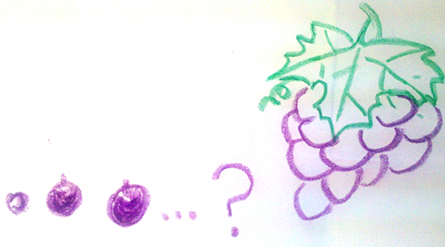
\includegraphics[scale=0.6]{img/grapes-1.eps}
  \caption{Always picking the smallest grape.} 
  \label{fig:eat-grapes}
\end{figure}

Based on this idea, the algorithm of selection sort can be directly
described as the following. 

In order to sort a series of elements:

\begin{itemize}
\item The trivial case, if the series is empty, then we are done, the result is also empty;
\item Otherwise, we find the smallest element, and append it to the tail of the result;
\end{itemize}

Note that this algorithm sorts the elements in increase order; It's easy to sort in decrease
order by picking the biggest element intead; We'll introduce about passing a comparator as
parameter later on.

This description can be formalized to a equation.

\be
sort(A) =  \left \{
  \begin{array}
  {r@{\quad:\quad}l}
  \Phi & A = \Phi \\
  \{ m \} \cup sort(A') & otherwise
  \end{array}
\right.  
\ee

Where $m$ is the minimum elenets among collection $A$, and $A'$ is all the rest elements
except $m$:

\[
\begin{array}{l}
m = min(A) \\
A' = A - \{ m \}
\end{array}
\]

We don't limit the data structure of the collection here. Typically, $A$ is array in imperative
environment, and list (singly linked-list particularly) in functional environment, and it can 
be even others as we introduced later.

The algorithm can also be given in imperative manner.

\begin{algorithmic}
\Function{Sort}{$A$}
  \State $X \gets \Phi$
  \While{$A \neq \Phi$}
    \State $x \gets$ \Call{Min}{$A$}
    \State $A \gets$ \Call{Del}{$A, x$}
    \State $X \gets$ \Call{Append}{$X, x$}
  \EndWhile
  \State \Return $X$
\EndFunction
\end{algorithmic}

Figure \ref{fig:sel-sort} dipicts the process of this algorithm.

\begin{figure}[htbp]
  \centering
  \includegraphics[scale=0.8]{img/sel-sort.ps}
  \caption{The left part is sorted data, continuously pick the minimum element in the rest and append it to the ressult.} 
  \label{fig:sel-sort}
\end{figure}

We just translate the very original idea of `eating grapes' line by line without
considering any expense of time and space cost. This realization store the result
in $X$, and when an selected element is appended to $X$, we delete the same element
from $A$. This indicates that we can change it to `in-place' sorting to reuse
the spaces in $A$.

The idea is to store the minimum element in the first cell in $A$ (we use term `cell' if
$A$ is array, and say `node' if $A$ is list); then store the second minimum element
in next cell, then third cell, ... 

One solution to realize this sorting strategy is swapping. When we select the $i$-th 
minimum element, we swap it with the element in the $i$-th cell:

\begin{algorithmic}
\Function{Sort}{$A$}
  \For{$i \gets 1$ to $|A|$}
    \State $m \gets$ \Call{Min}{$A[i...]$}
    \State \textproc{Exchange} $A[i] \leftrightarrow m$
  \EndFor
\EndFunction
\end{algorithmic}

Denote $A = \{a_1, a_2, ..., a_N\}$. At any time, when we process the $i$-th element, 
all elements before $i$, as $\{a_1, a_2, ..., a_{i_1}\}$ have already been sorted. 
We locate the minimum element among the $\{a_i, a_{i+1}, ..., a_N\}$, and exchange it
with $a_i$, so that the $i$-th cell contains the right value. The process is repeatedly
executed till we arrived at the last element. 

This idea can be illustrated by figure \ref{fig:in-place-sort}.

\begin{figure}[htbp]
  \centering
  \includegraphics[scale=0.8]{img/in-place-sort.ps}
  \caption{The left part is sorted data, continuously pick the minimum element in the rest and put it to the right position.} 
  \label{fig:in-place-sort}
\end{figure}

% ================================================================
% Find the minimum
% ================================================================
\section{Finding the minimum}
\index{selection sort!minimum finding}

We haven't completely realized the selection sort, because we take the operation
of finding the minimum (maximum) element as a black box. It's a puzzle how does
a kid locate the biggest or the smallest grape. 
And this is an interesting topic for computer algorithms.

The easist but not so fast way to find the minimum in a collection is to perform
a scan. There are several ways to interprete this scan process. Consider that
we want to pick the biggest grape. We start from any grape, compare it with 
another one, and pick the bigger one; then we take a next grape and compare
it with the one we selected so far, pick the bigger one and go on the take-and-compare
process, until there is no any grape we haven't compared.

It's easy to get loss in real practice if we don't mark which grape has been 
compared. There are two ways to to solve this problem, which are suitable for
different data-structures respectively.

\subsection{Labeling}
Method 1 is to label each grape with a number: $\{1, 2, ..., N\}$, and we systematically
perform the compare in the order of this sequence of labels. That we first 
compare grape number 1 and grape number 2, pick the bigger one; then we take grape
number 3, and do the comparation, ... We repeat this process until arrived at
grape number $N$. This is quite suitable for elements stored in an array.

\begin{algorithmic}
\Function{Min}{$A$}
  \State $m \gets A[1]$
  \For{$i \gets 2$ to $|A|$}
    \If{$A[i] < m$}
      \State $m \gets A[i]$
    \EndIf
  \EndFor
  \State \Return $m$
\EndFunction
\end{algorithmic}

With \textproc{Min} defined, we can complete the basic version of selection sort
(or naive version without any optimization in terms of time and space). 

However, this algorithm returns the value of the minimum element instead of its
location (or the label of the grape), which need a bit tweaking for the in-place version.
Some languages such as ISO C++, support returning the reference as result, so that the
swap can be achieved directly as below.

\lstset{language=C++}
\begin{lstlisting}
template<typename T>
T& min(T* from, T* to) {
    T* m;
    for (m = from++; from != to; ++from)
        if (*from < *m)
            m = from;
    return *m;
}

template<typename T>
void ssort(T* xs, int n) {
    int i;
    for (i = 0; i < n; ++i)
        std::swap(xs[i], min(xs+i, xs+n));
}
\end{lstlisting}

In environments without reference semantics, the solution is to return the location
of the minimum element instead of the value:

\begin{algorithmic}
\Function{Min-At}{$A$}
  \State $m \gets$ \Call{First-Index}{$A$}
  \For{$i \gets m + 1 $ to $|A|$}
    \If{$A[i] < A[m]$}
      \State $m \gets i$
    \EndIf
  \EndFor
  \State \Return $m$
\EndFunction
\end{algorithmic}

Note that since we pass $A[i...]$ to \textproc{Min-At} as the argument, we assume the first
element $A[i]$ as the smallest one, and examine all elements $A[i+1], A[i+2], ...$ one by one.
Function \textproc{First-Index}() is used to retrieve $i$ from the input parameter.

The following Python example program, for example, completes the basic in-place
selection sort algorithm based on this idea. It explicitly passes the range information
to the function of finding the minimum location.

\lstset{language=Python}
\begin{lstlisting}
def ssort(xs):
    n = len(xs)
    for i in range(n):
        m = min_at(xs, i, n)
        (xs[i], xs[m]) = (xs[m], xs[i])
    return xs

def min_at(xs, i, n):
    m = i;
    for j in range(i+1, n):
        if xs[j] < xs[m]:
            m = j
    return m
\end{lstlisting}

\subsection{Groupping}
Another method is to group all grapes in two parts: the group we have examined, and rest we
haven't. We denote these two groups as $A$ and $B$; All the elements (grapes) as $L$. 
At the beginning, we haven't examine any grapes at all, thus $A$ is empty ($\Phi$), and
$B$ contains all grapes. We can select arbitary two grapes from $B$, compare them, and 
put the loser (the smaller one for example) to $A$. After that, we repeat this process
by continously picking arbitrary grapes from $B$, and compare with the winner of the
previous time until $B$ becomes empty. At this time being, the final winner is the
minimum element. And $A$ turns to be $L - \{min(L)\}$, which can be used for the next
time minimum finding.

There is an invariant of this method, that at any time, we have $L = A \cup \{m\} \cup B$,
where $m$ is the winner so far we hold.

This approach doesn't need the collection of grapes being indexed (as being labeled
in method 1). It's suitable for any traversable data structures, including linked-list
etc. This method can be formalized as below.

\be
min(A, m, B) =  \left \{
  \begin{array}
  {r@{\quad:\quad}l}
  (m, A) & B = \Phi \\
  min(A \cup \{m\}, b_1, B') & b_1 < m \\
  min(A \cup \{b_1\}, m, B') & otherwise
  \end{array}
\right.  
\ee

TODO: stop at here.

TODO: Complexity analysis

All the insertion algorithms are bound to $O(N)$, where $N$ is the length of
the sequence. No matter what difference among them, such as scan from left
or from right. Thus the over all performance for insertion sort is quadratic
as $O(N^2)$.

\begin{Exercise}

\begin{itemize}
\item Provide explicit insertion function, and call it with general
insertion sort algorithm. Please realize it in both procedural way and
functional way.
\end{itemize}

\end{Exercise}

% ================================================================
% Improvement 1
% ================================================================

\section{Minor Improvement}
\index{Insertion sort!binary search}

TODO: iterate till |A|-1, but not |A|

Let's go back to the question, that why human being can find the proper
position for insertion so quickly. We have shown a solution based on scan.
Note the fact that at any time, all cards at hands have been well sorted,
another possible solution is to use binary search to find that location.

We'll explain the search algorithms in other dedicated chapter. Binary
search is just briefly introduced for illustration purpose here.

The algorithm will be changed to call a binary search procedure.

\begin{algorithmic}
\Function{Sort}{$A$}
  \For{$i \gets 2$ to \Call{Length}{$A$}}
    \State $x \gets A[i]$
    \State $p \gets $ \Call{Binary-Search}{$A[1...i-1], x$}
    \For{$j \gets i$ down to $p$}
      \State $A[j] \gets A[j-1]$
    \EndFor
    \State $A[p] \gets x$
  \EndFor
\EndFunction
\end{algorithmic}

Instead of scan elements one by one, binary search utilize the information
that all elements in slice of array $\{A_1, ..., A_{i-1} \}$ are sorted. 
Let's assume
the order is monotonic increase order. To find a position $j$ that satisfies
$A_{j-1} \leq x \leq A_{j}$. We can first examine the middle element, for 
example, $A_{\lfloor i/2 \rfloor}$. If $x$ is less than it, we need next recursively
perform binary search in the first half of the sequence; otherwise, we
only need search in last half.

Every time, we halve the elements to be examined, this search process runs
$O(\lg N)$ time to locate the insertion position.

\begin{algorithmic}
\Function{Binary-Search}{$A, x$}
  \State $l \gets 1$
  \State $u \gets 1+$ \Call{Length}{$A$}
  \While{$l < u$}
    \State $m \gets \lfloor \frac{l+u}{2} \rfloor$
    \If{$A_m = x$}
      \State \Return $m$ \Comment{Find a duplicated element}
    \ElsIf{$A_m < x$}
      \State $l \gets m+1$
    \Else
      \State $u \gets m$
    \EndIf
  \EndWhile
  \State \Return $l$
\EndFunction
\end{algorithmic}

The improved insertion sort algorithm is still bound to $O(N^2)$, 
compare to previous section, which we use $O(N^2)$ times comparison and
$O(N^2)$ moves, with binary search, we just use $O(N \lg N)$ times 
comparison and $O(N^2)$ moves.

The Python program regarding to this algorithm is given below.

\lstset{language=Python}
\begin{lstlisting}
def isort(xs):
    n = len(xs)
    for i in range(1, n):
        x = xs[i]
        p = binary_search(xs[:i], x)
        for j in range(i, p, -1):
            xs[j] = xs[j-1]
        xs[p] = x

def binary_search(xs, x):
    l = 0
    u = len(xs)
    while l < u:
        m = (l+u)/2
        if xs[m] == x:
            return m 
        elif xs[m] < x:
            l = m + 1
        else:
            u = m
    return l
\end{lstlisting}

\begin{Exercise}
Write the binary search in recursive manner. You needn't use purely functional
programming language.
\end{Exercise}

% ================================================================
% Improvement 2
% ================================================================

\section{Improvement 2}
\index{Insertion sort!linked-list setting}

Although we improve the search time to $O(N \lg N)$ in previous section, the
number of moves is still $O(N^2)$. The reason of why movement takes so long
time, is because the sequence is stored in plain array. The nature of array
is continuously layout data structure, so the insertion operation is expensive.
This hints us that we can use linked-list setting to represent the sequence.
It can improve the insertion operation from $O(N)$ to constant time $O(1)$.

\be
  insert(A, x) = \left \{
  \begin{array}
  {r@{\quad:\quad}l}
  \{ x \} & A = \Phi \\
  \{ x \} \cup A & x < A_1 \\
  \{ A_1 \} \cup insert(\{ A_2, A_3, ... A_n\}, x)& otherwise
  \end{array}
\right.  
\ee

Translating the algorithm to Haskell yields the below program.

\lstset{language=Haskell}
\begin{lstlisting}
insert :: (Ord a) => [a] -> a -> [a]
insert [] x = [x]
insert (y:ys) x = if x < y then x:y:ys else y:insert ys x
\end{lstlisting}

And we can complete the two versions of insertion sort program based on
the first two equations in this chapter.

\begin{lstlisting}
isort [] = []
isort (x:xs) = insert (isort xs) x
\end{lstlisting}

Or we can represent the recursion with folding.

\begin{lstlisting}
isort = foldl insert []
\end{lstlisting}

Linked-list setting solution can also be described imperatively. Suppose
function \textproc{Key}($x$), returns the value of element stored in node
$x$, and \textproc{Next}($x$) accesses the next node in the linked-list.

\begin{algorithmic}
\Function{Insert}{$L, x$}
  \State $p \gets NIL$
  \State $H \gets L$
  \While{$L \neq NIL \land $ \Call{Key}{$L$} $<$ \Call{Key}{$x$}}
    \State $p \gets L$
    \State $L \gets $ \Call{Next}{$L$}
  \EndWhile
  \State \Call{Next}{$x$} $\gets L$
  \If{$p \neq NIL$}
    \State $H \gets x$
  \Else
    \State \Call{Next}{$p$} $\gets x$
  \EndIf
  \State \Return $H$
\EndFunction
\end{algorithmic}

For example in ANSI C, the linked-list can be defined as the following.

\lstset{language=C}
\begin{lstlisting}
struct node{
  Key key;
  struct node* next;
};
\end{lstlisting}

Thus the insert function can be given as below.

\begin{lstlisting}
struct node* insert(struct node* lst, struct node* x){
  struct node *p, *head;
  p = NULL;
  for(head = lst; lst && x->key > lst->key; lst = lst->next)
    p = lst;
  x->next = lst;
  if(!p)
    return x;
  p->next = x;
  return head;
}
\end{lstlisting}

Instead of using explicit linked-list such as by pointer or reference
based structure. Linked-list can also be realized by another index array.
For any array element $A_i$, $Next_i$ stores the index of next element
follows $A_i$. It means $A_{Next_i}$ is the next element after $A_i$.

The insertion algorithm based on this solution is given like below.

\begin{algorithmic}
\Function{Insert}{$A, Next, i$}
  \State $j \gets \perp$
  \While{$Next_j \neq NIL \land A_{Next_j} < A_i$}
    \State $j \gets Next_j$
  \EndWhile
  \State $Next_i \gets Next_j$
  \State $Next_j \gets i$
\EndFunction
\end{algorithmic}

Here $\perp$ means the head of the $Next$ table. 
And the relative Python program for this algorithm is given as the following.

\lstset{language=Python}
\begin{lstlisting}
def isort(xs):
    n = len(xs)
    next = [-1]*(n+1)
    for i in range(n):
        insert(xs, next, i)
    return next

def insert(xs, next, i):
    j = -1
    while next[j] != -1 and xs[next[j]] < xs[i]:
        j = next[j]
    next[j], next[i] = i, next[j]
\end{lstlisting}

Although we change the insertion operation to constant time by using 
linked-list. However, we have to traverse the linked-list to find the
position, which results $O(N^2)$ times comparison. This is because
linked-list, unlike array, doesn't support random access. It means we
can't use binary search with linked-list setting.

\begin{Exercise}
\begin{itemize}
\item Complete the insertion sort by using linked-list insertion function
in your favorate imperative programming language.
\item The index based linked-list return the sequence of rearranged index
as result. Write a program to re-order the original array of elements from
this result.
\end{itemize}
\end{Exercise}

% ================================================================
% Final improvement
% ================================================================

\section{Final improvement by binary search tree}
\index{Insertion sort!binary search tree}

It seems that we drive into a corner. We must improve both the comparison 
and the insertion at the same time, or we will end up with $O(N^2)$ performance.

We must use binary search, this is the only way to improve the comparison
time to $O(\lg N)$. On the other hand, we must change the data structure, 
because we can't achieve constant time insertion at a position with 
plain array.

This remind us about our 'hello world' data structure, binary search tree.
It naturally support binary search from its definition. At the same time,
We can insert a new leaf in binary search tree in $O(1)$ constant time
if we already find the location.

So the algorithm changes to this.

\begin{algorithmic}
\Function{Sort}{$A$}
  \State $T \gets \Phi$
  \For{each $x \in A$}
    \State $T \gets $ \Call{Insert-Tree}{$T, x$}
  \EndFor
  \State \Return \Call{To-List}{$T$}
\EndFunction
\end{algorithmic}

Where \textproc{Insert-Tree}() and \textproc{To-List}() are described in 
previous chapter about binary search tree.

As we have analyzed for binary search tree, the performance of tree sort
is bound to $O(N \lg N)$, which is the lower limit of comparison based 
sort\cite{Knuth}.

\section{Short summary} 
In this chapter, we present the evolution process of insertion sort. Insertion
sort is well explained in most textbooks as the first sorting algorithm.
It has simple and straightforward idea, but the performance is quadratic.
Some textbooks stop here, but we want to show that there exist ways to improve
it by different point of view. We first try to save the comparison time
by using binary search, and then try to save the insertion operation by
changing the data structure to linked-list. Finally, we combine these
two ideas and evolute insertion sort to tree sort.

\begin{thebibliography}{99}

\bibitem{wiki-bubble-sort}
http://en.wikipedia.org/wiki/Bubble\_sort

\bibitem{CLRS}
Thomas H. Cormen, Charles E. Leiserson, Ronald L. Rivest and Clifford Stein. 
``Introduction to Algorithms, Second Edition''. ISBN:0262032937. The MIT Press. 2001

\bibitem{Knuth}
Donald E. Knuth. ``The Art of Computer Programming, Volume 3: Sorting and Searching (2nd Edition)''. Addison-Wesley Professional; 2 edition (May 4, 1998) ISBN-10: 0201896850 ISBN-13: 978-0201896855

\end{thebibliography}

\ifx\wholebook\relax\else
\end{document}
\fi
